\documentclass[a4paper,11pt]{article}
\usepackage[pdftex]{graphicx}
\usepackage{color}
\usepackage[top=2cm, bottom=2cm, margin=2cm]{geometry}
\usepackage{longtable}
\usepackage{fancyhdr}
\usepackage{tikz}
\usepackage{mirantis}
\usepackage{booktabs}
\usepackage{tabularx}

\begin{document}

\thispagestyle{empty}
\titleGWP{Savanna Test Plan}{}

\clearpage

\pagestyle{fancy}
\thispagestyle{fancy}

\tableofcontents

\newpage

\section{Revision History}

\begin{tabular}{|l|p{4cm}|p{10cm}|}
\hline
{\bf Date} & {\bf Author} & {\bf Comments} \\ 
\hline
12/03/2013 & QA team & Initial Draft \\ 
\hline
\end{tabular}





\section{Introduction}

The main goal of this document is to present a detailed test cases for Savanna testing. This test plan includes functional test cases for the features and non-functional test cases for performance, load and compatibility testing types. This document is divided to sections by the testing types. 





\section{System Under Test Specifications}

\begin{itemize}
\item TBD
\end{itemize}





\section{QA Team Responsibilities}

QA team is responsible to:
\begin{itemize}
\item make a test plan contains acceptance, functional, performance, scalability, reliability and compatibility test cases
\item add regression test cases to the test plan in case of regression
\item define acceptance tests suite for every iteration
\item execute acceptance tests for candidate build for every iteration
\item execute acceptance and regression tests for release candidate
\item execute all functional, scalability, reliability and compatibility test cases on stable nightly builds when corresponding features will be implemented
\item maintain test lab infrastructure
\item automate as many acceptance tests as possible
\item execute automated test suite for each nightly build
\item maintain infrastructure for making nightly builds and run automated tests
\item notify Dev team about found bugs via bug tracking system
\item help Dev team with bug reproduction
\item verify bugs fixed by Dev team
\end{itemize}

\subsection{Test Deliverables}
The following items should be delivered after product release:
\begin{enumerate}
\item test plan
\item test cases specification
\item test cases execution reports
\item project status and metrics
\end{enumerate}

\subsection{Test Schedule}
\begin{enumerate}
\item TBD
\end{enumerate}

\subsection{Test Cycles}
\begin{enumerate}
\item Implemented functionality (pass 1)
\item Working functionality (pass 2)
\item All critical bugs and bugs related to functionality fixed - acceptance for demo (pass 3)
\end{enumerate}





\section{Suspension Criteria and Resumption Requirements}

The main criteria to suspend the testing for candidate build is having at least one 'Blocker' bug. Resumption criteria in that case is fixing all 'Blocker' bugs and make a new candidate build.
Performance testing can be suspended if the product is unstable on the load. Resumption criteria for that case is fixing corresponding bugs and make a new stable build.





\section{Risk Areas Evaluation}

Risk Areas were evaluated by their severity and priority. These potential risks will be addressed by tests. Number of test cases for each feature is determined by the priorities defined on the basis of severity and probability of risks, related to this feature.

Each test case has a priority according to and probability of a particular risk, related to this test case. Also each test case has a priority for automation.

\newpage
\begin{longtable}{|c|p{3cm}|c|c|p{8cm}|}
\hline
\# & {\bf Risk} & {\bf Severity} & {\bf Probability} & {\bf Comments}\\
\hline
1&Difference between REST API requirements and implementation& High & Low & The following items must be tested:
\begin{itemize}
\item Node template requests: create, modify, delete
\item Cluster requests: create, modify, delete
\end{itemize}
\\ \hline
2&Errors in the REST API implementation& High & High & The following items must be tested:
\begin{itemize}
\item Deploy acceptance
\item Hadoop acceptance
\end{itemize}
\\ \hline
3&Errors in the plugin API functionality & High & High & REST API requests should be tested for the following Hadoop implementations:
\begin{itemize}
\item Apache Hadoop
\item Hortonworks Ambari
\item Clouderra Manager
\item Intel Hadoop
\end{itemize}
\\ \hline
4&Errors in the UI functionality & High & High & The following items must be tested:
\begin{itemize}
\item Node template requests through Horizon UI: create, modify, delete
\item Cluster requests through Horizon UI: create, modify, delete
\item TBD
\end{itemize}
\\ \hline
5&Savanna is not compatible with custom Hadoop images & Medium & High & Create a Hadoop cluster using Hadoop images provided by Hortonworks Ambari, 
Clouderra Manager, Intel Hadoop, etc \\ \hline
6&Savanna is not compatible with different OpenStack releases& Medium & High & Savanna should be installed on the upcoming OpenStack releases(TBD which) \\ \hline
7&Savanna is not compatible with different versions of Python& High & High & Savanna should be tested on Python 2.6 and 2.7. Also it should be tested on 3.x versions when the OpenStack does support them. \\ \hline
8&Installation problems& High &  Low & Savanna supports 2 installation modes: from the sources and using pip utility. Both of them should be tested.\\ \hline
9&Lack of UI performance & Medium & Medium & TBD \\ \hline
10&Low performance of Hadoop deploying & Medium & Medium & TBD\\ \hline
11&Low performance of Apache Hadoop HDFS & Medium & Medium & TBD\\ \hline
12&Low performance of Apache Hadoop MapReduce & Medium & Medium & The following scenarios must be tested:
\begin{itemize}
\item Pi evaluation
\item Load test script(TBD name?)
\end{itemize}
\\ \hline
\end{longtable}





\section{Features To Be Tested}
%\subsection{TBD}
\textbf{Basic Cluster Provisioning}

\begin{itemize}
    \item Cluster provisioning
    \item Deployment Engine implementation for pre-installed images
    \item Templates for Hadoop cluster configuration
    \item REST API for cluster startup and operations
    \item UI integrated into Horizon
\end{itemize}
\textbf{Cluster Operations}

\begin{itemize}
    \item Manual cluster scaling (add/remove nodes)
    \item Hadoop cluster topology configuration parameters
	\begin{itemize}
    		\item Data node placement control
        \item HDFS location
        \item Swift integration
    \end{itemize}

    \item Integration with vendor specific deployment/management tooling
    \item Monitoring support - integration with 3rd-party monitoring tools (Zabbix, Nagios)
\end{itemize}
\textbf{Analytics as a Service}

\begin{itemize}
    \item API to execute Map/Reduce jobs without exposing details of underlying infrastructure (similar to AWS EMR)
    \item User-friendly UI for ad-hoc analytics queries based on Hive or Pig
\end{itemize}
\textbf{Further Roadmap}
\begin{itemize}
    \item HDFS and Swift integration
	\begin{itemize}
    		\item Caching of Swift data on HDFS
        \item Avoid issues with Swift eventual consistency while running job
	\end{itemize}
    \item HBase support
\end{itemize}





\section{Features NOT to be tested}

\begin{tabular}{|p{5cm}|p{10cm}|}
\hline
\ \bf Feature & \bf Reason \\ \hline
TBD&TBD \\ \hline
\end{tabular}





\newpage
\section{Test lab network topology}

\subsection{Descriptions of network topology and servers destination}
\paragraph{} Virtualized infrastructure is used for Savanna testing presented on the Figure 1.
\begin{itemize}
\item \textit{Switch} - usual a switch-device.
\item \textit{Swift node} - on this nodes can run the virtual machine.
\item \textit{Management node} - this node manage lab.
\item \textit{Compute node} - on this node run the virtual machines.
\end{itemize}

\subsection{Network scheme for tests}
This scheme is used in all test cases for Savanna.

\begin{figure}[hb]
\caption{Network scheme for tests}
 \begin{center}
  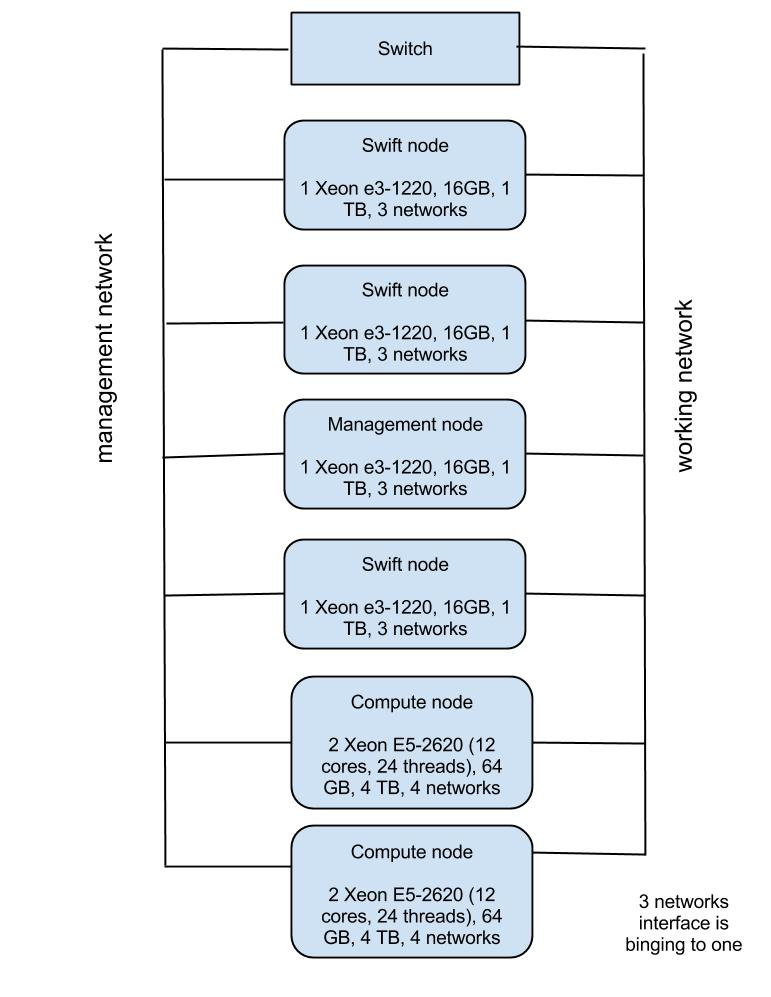
\includegraphics[width=9cm]{HadoopLabSchema.jpg}
 \end{center}
\label{fig:MainScheme}
\end{figure}





\section{Test Cases Requirements}

\begin{itemize}
\item All possible test cases should be automated.
\item At least 70\% of the test cases should be automated.
\end{itemize}

\end{document}
